\documentclass[a4paper]{article}

\usepackage[utf8]{inputenc}
\usepackage{graphicx}
\usepackage{titlepic}
\usepackage{textcomp}
\usepackage{tabularx}
\usepackage{float}
\usepackage{hyperref}
\usepackage{datetime}
\usepackage{xurl}
\hypersetup{
    colorlinks=true,
    linkcolor=blue,
    filecolor=magenta,
    urlcolor=cyan,
}
\setlength{\parindent}{0pt}

\urlstyle{same}

\graphicspath{{./images}}

%opening
\title{Authentication Project: 2FA Using Usernames, Passwords and Time-based One-time Passwords}
\titlepic{
\includegraphics[width=0.25\textwidth]{ju.png}}
\author{Ward M. Zahran}

\begin{document}

\maketitle
\pagebreak

\tableofcontents
\pagebreak

\section{Team Members}
\begin{enumerate}
    \item Ward M. Zahran.
\end{enumerate}

\section{Brief Description}
This project aims to implement user two-factor authentication for a web application using usernames and password along with time-based one-time passwords as a second factor. 

The project uses Go and SQlite3 and TOTP as defined in RFC 6238.

\section{Primer on How TOTP Works}
TOTP (Time-Based One-Time Password) is an algorithm defined in RFC 6238 which extends the HOTP (HMAC-Based One-Time Password) as defined in RFC 4226. We will explain the latter then explain the former.

\subsection{HOTP}

HOTP defines the following symbols:
\begin{itemize}
    \item 
        A symetric secret key (K).
    \item 
        A hash function (H) the default being SHA-1.
    \item 
        A counter value (C) in order to generate one time passwords.
    \item 
        A HOTP value length (D) (6–10, default is 6, and 6–8 is recommended).
\end{itemize}

These values must be agreed upon by both parties, in our case the webapp and the user. 

The algorithm uses the following formula in order to get a HOTP value: \\

$ HOTP  value = HOTP(K, C) mod 10^D$ \\
$ HOTP(K, C) = truncate(HMACH(K, C))$ \\
$ truncate(MAC) = extract31(MAC, MAC[(19 × 8 + 4):(19 × 8 + 7)])$ \\
$ extract31(MAC, i) = MAC[(i × 8 + 1):(i × 8 + 4 × 8 − 1)]$ \\



\begin{enumerate}
    \item 
        We generate a HOTP value from the HTOP(K, C) modulo 10 to the power of the key length D.
    \item 
        The HOTP function first generates the HMAC using K and C and then truncates it.
    \item 
        The truncate function does some math on the hash and then produces the value. 
    \item 
        Once the value generated both parties increment the counter C independently.
\end{enumerate}

\subsection{TOTP}

TOTP uses the same exact algorithm but instead of a counter we use a new value based on time which we will call T. 

So our algorithm ends up being:
$HOTP  value = HOTP(K, T) mod 10^D$ \\



Per RFC 6238:

T = (Current Unix time - T0) / X

where:

\begin{itemize}
    \item 
        T0 is is the Unix time to start counting time steps (default value is 0, i.e., the Unix epoch). Meaning an agreed upon time from which to start counting the time.
    \item 
        X is the time step in seconds (default value X = 30 seconds). Meaning the amount of time before each code changes.
\end{itemize}

\section{Implementation}
My implementaiton was using Go with several libraries most important of which are the SQLite3, otp, http. 
As well as libraries we used various technologies in order to prevent automated attacks such as Captcha.

The user can register a new account through the following protal:

\begin{figure}[H]
    \begin{center}
        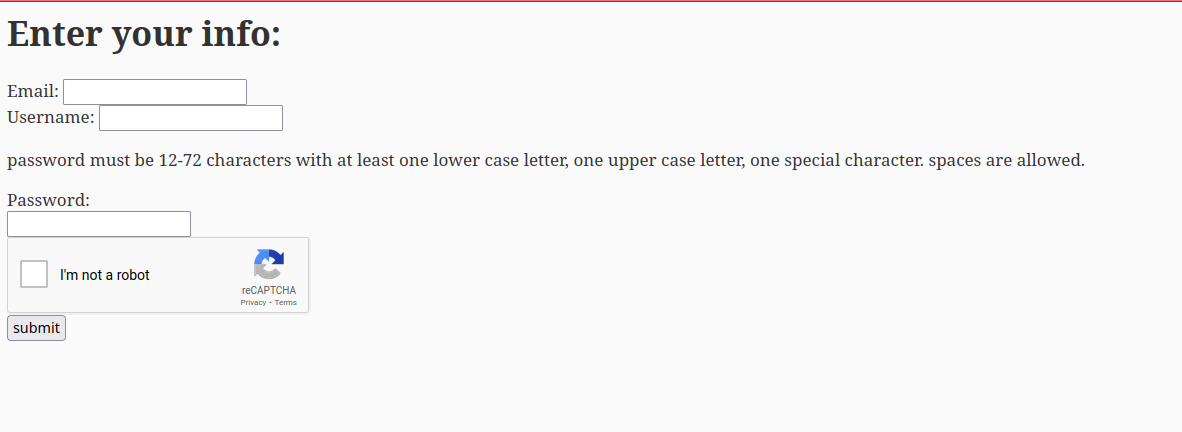
\includegraphics[width=0.95\textwidth]{reg.png}
    \end{center}
    \caption{User registration.}\label{fig:}
\end{figure}

Notice how we have implemented a captcha to disable autommated attacks from flodding the database with garbage information.

After the registration is done and user tries to login they will be faced with this page:

\begin{figure}[H]
    \begin{center}
        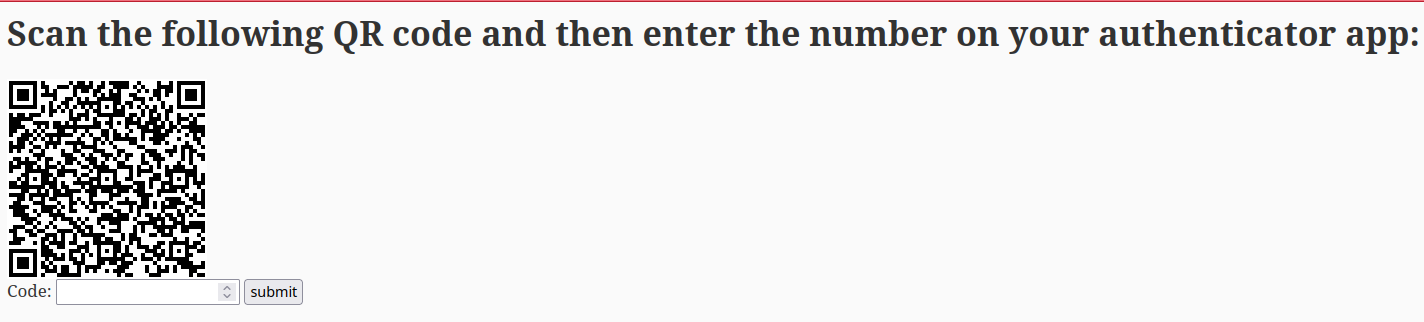
\includegraphics[width=0.95\textwidth]{auth_app.png}
    \end{center}
    \caption{2FA setup page}\label{fig:}
\end{figure}

The user cant access the rest of the website until he has scanned the QR code and used the OTP.

And on every subsequent login they will be faced with a different page without the QR code where they must enter the OTP. Notice the following figure:

\begin{figure}[H]
    \begin{center}
        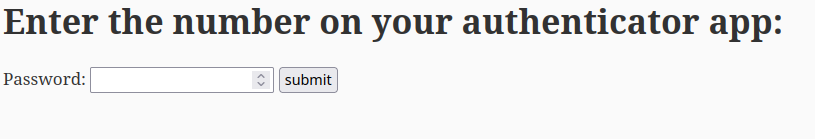
\includegraphics[width=0.95\textwidth]{login.png}
    \end{center}
    \caption{Login after verification.}\label{fig:}
\end{figure}

The workflow of how the login process works are as follows:

\begin{figure}[H]
    \begin{center}
        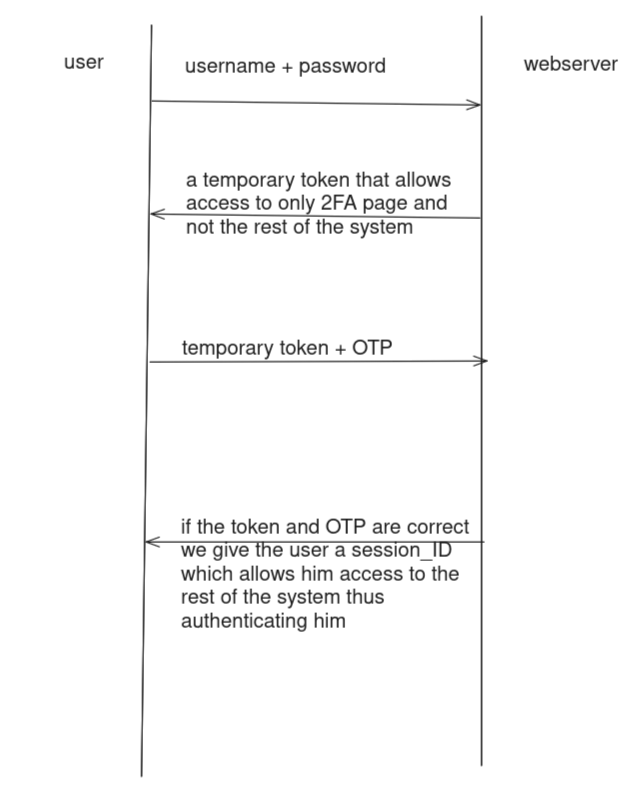
\includegraphics[width=0.95\textwidth]{control_flow.png}
    \end{center}
    \caption{Control flow}\label{fig:}
\end{figure}

After 3 invalid submissions the temporary token is invalidated thus protecting the system from brute force attacks. And aquiring a new temporary token is to automate because of the Captcha at the login page.


Other protections include Cron Jobs which automatically remove any unverified users at every midnight as well as purgin expired tokens and sessions.

\begin{figure}[H]
    \begin{center}
        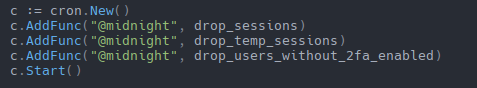
\includegraphics[width=0.95\textwidth]{cron.png}
    \end{center}
    \caption{Cron Jobs.}\label{fig:}
\end{figure}

\begin{figure}[H]
    \begin{center}
        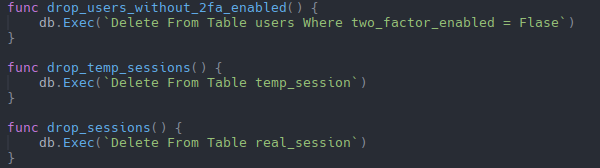
\includegraphics[width=0.95\textwidth]{cronfunc.png}
    \end{center}
    \caption{The functions run in those Cron jobs.}\label{fig:}
\end{figure}

As well as that we use envoriment variables rather than hard coding credentails into the server itself which protects them incase the software itself gets leaked.

\end{document}
